For the Petri net



\begin{centering}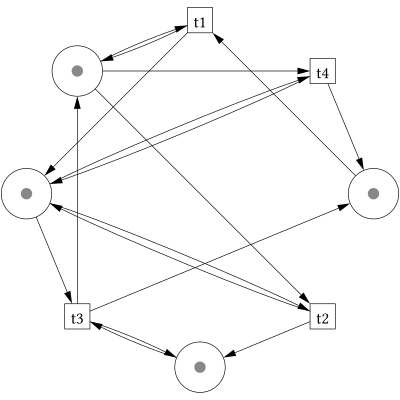
\includegraphics[min width=0.4\textwidth=0.6\textwidth,min height=0.4\textwidth=0.6\textwidth,keepaspectratio,max width=0.9\textwidth,max height=0.9\textwidth]{60/graph-1petri6798dd80b41d3221abe8bfcf7931ecef48ab6bc5eebe09d6a77c220768a60f7501013.pdf}\end{centering}

a transition sequence is sought which leads to the following marking:

\begin{centering}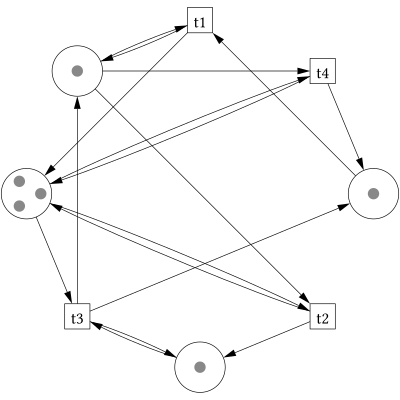
\includegraphics[min width=0.4\textwidth=0.6\textwidth,min height=0.4\textwidth=0.6\textwidth,keepaspectratio,max width=0.9\textwidth,max height=0.9\textwidth]{60/graph0petri18a6832a0ea325f8b83c352cdac8b029dd3b900696e925eeb0e69da1c00473ec01013.pdf}\end{centering}





State your solution as a sequence of the following kind that does not exceed 8 steps:


\begin{minted}{text}
[t1, t2, t3]
\end{minted}
Where giving these three steps means that after firing t1, then t2, and finally t3 (in exactly this order), the sought marking is reached.

Hint: There is no solution with less than 8 steps.

Please note: When hovering over or clicking on edges / nodes or their labels, the respective components that belong together are highlighted.